\documentclass[10pt,twocolumn]{article}

\usepackage[margin=0.72in]{geometry}
\usepackage[T1]{fontenc}
\usepackage{amsmath,amssymb}
\usepackage{booktabs}
\usepackage{graphicx}
\usepackage{xurl}
\usepackage[hidelinks]{hyperref}
\usepackage{enumitem}
\usepackage{balance}
\usepackage{pgfplots}
\pgfplotsset{compat=1.17}

\setlength{\columnsep}{0.24in}
\setlist{nosep,leftmargin=*}
\title{Measured Kernel and Speculative-Head Optimizations for Local LLM Inference on the SpaceMiT K1}
\author{Project report}
\date{24 September 2026}

\begin{document}
\maketitle

\begin{abstract}
This report evaluates low-level inference optimizations in the project for the SpaceMiT K1 system-on-chip, tested on a MUSE-Pi-Pro board. The work combines an IME1 matrix-kernel path for Q8\_0 weights, a register-level optimization to the IME Q4\_0 scale construction, and a mapped multi-token-prediction (MTP) speculative head. Experiments are reported at both kernel and end-to-end levels. On the 4B workload, Q8\_0 IME1 raises prompt processing from 1.117 to 7.472 tokens/s and generation from 0.866 to 1.349 tokens/s relative to its measured baseline. The M4 scale change raises 4B Q4\_0 prompt throughput by 3.3\%, while generation is unchanged. On the mapped 2B MTP workload, the same change adds about 1.8\% throughput in English and Chinese with matching acceptance counts and output hashes. A candidate Chinese vocabulary map did not improve held-out performance. A speculative timing gate and a hybrid IME/RVV dispatch were also evaluated and rejected after regressions. The report also logs the preceding optimization chain on the same fork---TCM runtime linkage, recurrent-state write-back, multi-token-prediction speculative decoding with truncated and mapped draft heads, and concurrency-adaptive gating---which raised 2B single-stream decode from 3.07 to 6.31 tokens/s and 4B from 2.23 to 3.20 tokens/s, with speculative output identical to direct decoding on the tested prompts. A speculative timing gate and a hybrid IME/RVV dispatch were also evaluated and rejected after regressions. The results show that the largest measured benefit comes from making an existing matrix path usable for Q8\_0; smaller kernel changes produce modest end-to-end gains, while proposal-cost overhead can erase speculative-decoding gains.
\end{abstract}

\begin{figure*}[t]
\centering
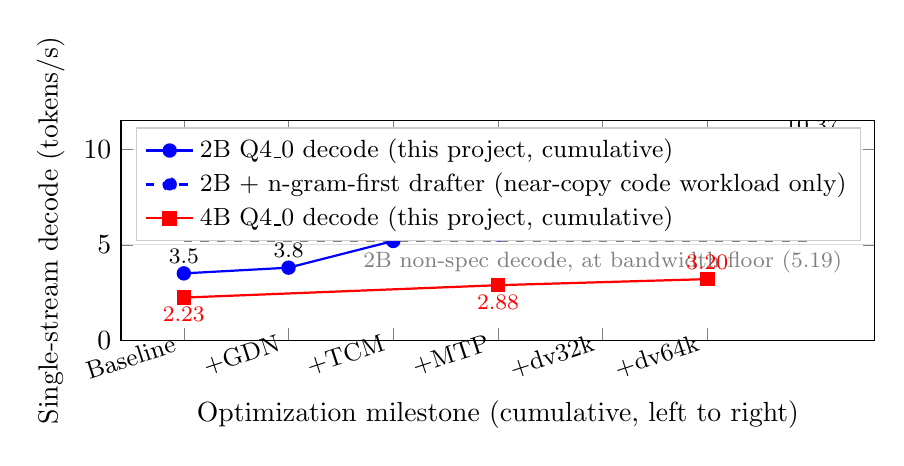
\begin{tikzpicture}
\begin{axis}[
  width=0.92\textwidth, height=0.36\textwidth,
  xlabel={Optimization milestone (cumulative, left to right)},
  ylabel={Single-stream decode (tokens/s)},
  symbolic x coords={Baseline, +GDN, +TCM, +MTP, +dv32k, +dv64k, +ngram},
  xtick=data, x tick label style={font=\small, rotate=18, anchor=east},
  ymin=0, ymax=11.5,
  ymajorgrids=true, grid style={gray!25},
  legend style={at={(0.02,0.97)}, anchor=north west, font=\small, draw=gray!40},
  legend cell align={left},
  mark size=2.2pt,
]
% ---- 2B chain ----
\addplot[color=blue, mark=*, thick] coordinates {
  (Baseline,3.5) (+GDN,3.8) (+TCM,5.2) (+MTP,5.54) (+dv32k,5.87) (+dv64k,6.31)
};
\addlegendentry{2B Q4\_0 decode (this project, cumulative)}
% ---- 2B ngram extension (workload-specific) ----
\addplot[color=blue, mark=*, thick, dashed] coordinates {
  (+dv64k,6.31) (+ngram,10.37)
};
\addlegendentry{2B + n-gram-first drafter (near-copy code workload only)}
% ---- 4B chain ----
\addplot[color=red, mark=square*, thick] coordinates {
  (Baseline,2.23) (+MTP,2.88) (+dv64k,3.20)
};
\addlegendentry{4B Q4\_0 decode (this project, cumulative)}
% ---- non-spec floor reference ----
\addplot[color=gray, dashed, domain=0:6, forget plot] coordinates {
  (Baseline,5.19) (+ngram,5.19)
};
\node[font=\footnotesize, color=gray, anchor=north] at (axis cs:+dv32k,5.19) {2B non-spec decode, at bandwidth floor (5.19)};
% value labels on 2B chain
\node[font=\footnotesize, anchor=south] at (axis cs:Baseline,3.5) {3.5};
\node[font=\footnotesize, anchor=south] at (axis cs:+GDN,3.8) {3.8};
\node[font=\footnotesize, anchor=south] at (axis cs:+TCM,5.2) {5.2};
\node[font=\footnotesize, anchor=south west] at (axis cs:+MTP,5.54) {5.54};
\node[font=\footnotesize, anchor=south] at (axis cs:+dv32k,5.87) {5.87};
\node[font=\footnotesize, anchor=south] at (axis cs:+dv64k,6.31) {6.31};
\node[font=\footnotesize, anchor=south] at (axis cs:+ngram,10.37) {10.37};
\node[font=\footnotesize, anchor=north, color=red] at (axis cs:Baseline,2.23) {2.23};
\node[font=\footnotesize, anchor=north, color=red] at (axis cs:+MTP,2.88) {2.88};
\node[font=\footnotesize, anchor=south, color=red] at (axis cs:+dv64k,3.20) {3.20};
\end{axis}
\end{tikzpicture}
\caption{Single-stream decode throughput across the optimization chain on the MUSE-Pi-Pro (llama-server, 4 threads, flash attention, greedy, output verified identical to direct decoding). Solid lines are cumulative milestones on the same workload; the dashed 2B extension is the n-gram-first combined drafter, which applies to copy-heavy code-editing workloads only. The gray reference marks the non-speculative 2B decode, which already sits at the measured memory-bandwidth floor; all gains above it come from drafting more than one token per target-model pass.}
\label{fig:chain}
\end{figure*}

\section{Introduction}
The project investigates local language-model inference on the SpaceMiT K1, whose X60 CPU cores provide RISC-V Vector support and a vendor Integer Matrix Extension (IME). The engineering question is which published or publicly available optimization ideas lead to measurable user-level gains on this constrained platform.

The work considered three layers: (1) matrix multiplication and quantized weight kernels, (2) draft-head vocabulary projection and speculative decoding, and (3) context growth and memory cost. The implementation and measurements target the MUSE-Pi-Pro K1 board and llama.cpp-derived code. Results should therefore be read as board-specific measurements, not as a general characterization of all K1 devices.

\section{Platform and evaluation method}
The target was a MUSE-Pi-Pro based on the SpaceMiT K1/X60. The evaluated models were Qwen3.5-2B and Qwen3.5-4B conversational checkpoints, distributed as GGUFs and augmented or requantized for MTP experiments. Their project filenames omit the word ``Instruct''; they are distinct from the separately published ``-Base'' checkpoints~\cite{qwen35_2b,qwen35_4b}. The principal throughput measurements use llama-bench prompt processing (pp) and token generation (tg); the report records pp64, pp128, and tg32 cases where applicable. Speculative decoding was evaluated with an attached draft head and target-model verification. A/B runs were interleaved for the M4 and vocabulary-map comparisons to reduce sensitivity to board contention.

For output-preservation checks, three short greedy server prompts (English, Chinese, and code) were run with baseline and modified Q8\_0 kernels and compared using output SHA-256 hashes. MTP comparisons also tracked accepted-token counts and output hashes. Matching hashes establish equality for those particular prompts and settings; they are not a proof of bitwise equivalence for all inputs or sampling configurations.

The exact commands, raw JSONL measurements, patch series, and board integration record are kept alongside this report in the project report and raw-measurement directories. Reported improvements are ratios or percentage differences from the corresponding measured baseline; distinct model, quantization, and prompt workloads are not combined into a single score.

\section{Step-by-step optimization log}
The kernel work in Section~\ref{sec:methods} sits on top of a longer optimization chain executed on the official SpaceMiT llama.cpp fork (branch \texttt{port-gdn}). This section records what was done at each step, in order, with the measured effect of each step; Figure~\ref{fig:chain} plots the cumulative decode-throughput chain. Unless noted, numbers are 2B Q4\_0 single-stream decode tokens/s (llama-server, 4 threads, flash attention, microbatch 32, greedy); ``bench'' numbers are llama-bench tg128/pp128. All speculative configurations below were verified output-identical to non-speculative greedy decoding on the tested prompts.

\begin{enumerate}[label=\textbf{Step \arabic*.},leftmargin=3.2em]
\item \textbf{Roofline accounting.} The 2B model moves 1.061\,GB of weights plus 37.7\,MB of recurrent state per token; at the measured $\approx$5.26\,GB/s effective memory bandwidth this gives a $\approx$209\,ms/token floor ($\approx$4.8\,tok/s). Every later decode number was read against this roofline, and the single-stream result ended within $\approx$6\% of it.
\item \textbf{GDN state in-place write-back + fused RVV decode} (commit \texttt{f106a7d}, ported from the research branch). The hybrid Qwen3.5 architecture runs 18 gated-delta-net (SSM) layers; this removed one $\approx$1\,MB state round-trip per layer per token. Official fork: 3.5 $\to$ 3.8\,tok/s.
\item \textbf{TCM runtime linkage fix.} The spert runtime probes \texttt{libspine\_tcm.so} by weak symbol and \emph{silently} falls back to DDR tile buffers when it is absent from \texttt{LD\_LIBRARY\_PATH}. Measured tile bandwidth: real TCM write 24.7 / read 9.26\,GB/s versus DDR fallback 2.2 / 5.2\,GB/s. Adding the library: 3.8 $\to$ 5.2\,tok/s --- the single largest fix in the project, and a configuration trap rather than a code change.
\item \textbf{MTP speculative decoding enabled.} Qwen3.5 ships one multi-token-prediction layer; enabling it with a full-vocabulary draft head gave 5.54\,tok/s at acceptance length 3.07, greedy output identical to direct decoding.
\item \textbf{Truncated draft-vocabulary head (dv64k).} The draft lm\_head dominated draft cost (286\,MB per draft token for 2B). A GGUF surgery appended a head holding only the first 65{,}536 embedding rows; the graph pads the missing logits with $-\infty$, so verification still uses the full vocabulary and the scheme is lossless by construction. Result: \textbf{6.31\,tok/s} (+22\% over the 5.19 non-speculative decode). A draft-length sweep confirmed n\_max\,=\,3 as optimal (2/4/5 all slower).
\item \textbf{Multi-stream crossover and adaptive gate.} Speculation was found to win at concurrency $\leq$2 (bandwidth-bound) and lose at $\geq$4 (IME-compute-bound), because the recurrent rollback snapshots also disabled the Step-2 fast path. Fixes: a server-side gate (\texttt{SPINE\_SPEC\_MAX\_ACTIVE}, default 1) that stops drafting when several slots are active, and a default switch from snapshot rollback to checkpoint rollback. Aggregate throughput at concurrency 8: 9.85 $\to$ \textbf{13.85\,tok/s}, matching the non-speculative 13.49 while keeping single-stream at 5.40 by default (6.31 with snapshot rollback for dedicated single-stream use).
\item \textbf{Prompt-processing microbatch sweet spot.} Block-GEMM scheduling degrades at M$\geq$64; setting \texttt{-ub 32} raised pp128 from 13.03 to \textbf{22.07\,tok/s} (+69\%), a configuration-only change that does not affect decode.
\item \textbf{4B MTP head from scratch.} The published 4B Q4\_0 GGUF lacks MTP tensors, so they were extracted from the Hugging Face repository with HTTP range requests (241\,MB of bf16) and surgically inserted into the quantized GGUF. Two non-obvious conventions had to be matched: the GGUF \texttt{block\_count} includes the MTP layer (32$\to$33), and all norm weights are stored zero-centered (converter adds $+1$); omitting the offset made the draft produce 0/375 accepted tokens. With the offset fixed and a 64k truncated head, 4B single-stream went 2.23 $\to$ \textbf{3.20\,tok/s} (+43\%), output-identical to direct decoding; 4B non-speculative decode (2.30) already sits at the bandwidth floor.
\item \textbf{Frequency-mapped 32k draft head (d2t).} Replacing the prefix rows with the 32k most frequent token IDs (map trained on 809k corpus tokens) kept English/code gains and repaired the prefix head's weakness on Chinese: 3.58 $\to$ 4.92\,tok/s (+37.6\%).
\item \textbf{Low-acceptance fallback} (commit \texttt{f3e71c9}, \texttt{SPINE\_SPEC\_LOW\_ACC}). On low-acceptance prompts speculation was a \emph{negative} optimization (3.7--4.2 versus 5.09 direct); the slot now disables its own drafting after twelve verification rounds below 75\% acceptance, recovering direct-decoding speed automatically.
\item \textbf{N-gram-first combined speculation} (configuration only). \texttt{--spec-type ngram-mod,draft-mtp} with 16-token match drafting reached \textbf{10.37\,tok/s} on a near-copy C++ edit versus 7.99 with MTP alone (+29.7\%), and 3.63 versus 3.39 (+7.2\%) on 4B; prose workloads were unchanged.
\item \textbf{Q8\_0 IME1 kernel and M4 scale rewrite} (commit \texttt{a990751}, Section~\ref{sec:methods}): 4B Q8\_0 pp $6.69\times$, 4B Q4\_0 pp +3.3\%.
\end{enumerate}

\paragraph{Measured and rejected.} Quantization below Q4\_0 (no IME kernels; pre-kernel Q8\_0 measured pp 1.12 / tg 0.87), IME2/q2\_k routes (\texttt{use\_ime2: 0} on this board), TCM tile staging re-layouts (neutral or regressive), spert runtime environment knobs (no measurable effect), a hybrid IME/RVV dispatch (2B tg 5.16 $\to$ 2.01), and a first-twelve-rounds speculation timing gate (disabled a beneficial configuration; see Section~\ref{sec:methods}) were all evaluated and excluded.

\section{Optimization methods}
\label{sec:methods}
\subsection{Q8\_0 IME1 matrix kernel}
The first optimization enables the SpaceMiT IME1 matrix-multiply path for Q8\_0 weights, based on the llama.cpp change in pull request \#28479~\cite{llamacpp_q8_ime}. This creates a usable IME execution route for a higher precision quantization than Q4\_0. The project packaged the change as an opt-in patch so it can be applied independently and compared against the existing kernel selection.

\subsection{M4 block-scale construction}
The Q4\_0 IME kernel performs integer matrix operations and applies per-block scales. The evaluated M4 patch rewrites the scale build using eight vector-vector multiplies and prebuilt row-scale vectors in place of sixteen masked vector-scalar multiplies and four vector moves. The upstream study reports bit-exact kernel output and an isolated-kernel improvement; this project measures its effect in end-to-end inference on the K1~\cite{x60_scale_study}.

\subsection{Mapped MTP vocabulary head}
The project also evaluates MTP speculative decoding with a mapped draft-head vocabulary projection. The public Chinese vocabulary map was generated from the available Qwen and SpaceMiT tokenizer/model metadata and packaged as an experimental asset. Mapping limits head work to a subset of target vocabulary rows, intended to reduce draft-projection cost while preserving candidate usefulness. The evaluated map is a candidate configuration, not a default, because held-out measurements did not show a durable gain.

\subsection{Rejected alternatives}
Two additional approaches were measured. A timing gate estimated the rate of draft-and-verify rounds and disabled speculation when measured throughput fell below a direct-decoding threshold. A hybrid dispatch attempted to mix the IME and RVV routes. Both were kept out of the integrated result because they regressed relevant workloads. Recent adaptive speculative-decoding work motivates cost-aware policies~\cite{learning_to_draft,adasd}, but these experiments show that a simple online gate can make a poor decision when its initial window is noisy or not representative.

\section{Results}
\subsection{Q8\_0 IME1}
Table~\ref{tab:q8} shows the largest positive result. On the 4B Q8\_0 workload, prompt-processing throughput increased by a factor of 6.69 and generation throughput by 55.8\%. Q4\_0 control workloads were approximately unchanged, which is consistent with the patch affecting the Q8\_0 route rather than generally accelerating the model.

\begin{table}[t]
\centering
\caption{4B Q8\_0 throughput before and after enabling IME1.}
\label{tab:q8}
\begin{tabular}{lrrr}
\toprule
Metric & Baseline & IME1 & Change \\
\midrule
pp64 (tok/s) & 1.117 & 7.472 & $6.69\times$ \\
tg32 (tok/s) & 0.866 & 1.349 & $+55.8\%$ \\
\bottomrule
\end{tabular}
\end{table}

The prompt-processing gain is much larger than the generation gain, indicating that the matrix path changes the compute-heavy prompt phase more strongly than the token-by-token phase. In the tested short greedy prompts, all three output hashes matched the baseline. The board report retains Q4\_0 as the faster and smaller general-purpose path; Q8\_0 is useful when its precision/storage trade-off is desired and its IME route is enabled.

\subsection{M4 scale optimization}
Table~\ref{tab:m4} reports the end-to-end effects. For the 4B Q4\_0 path at pp128, throughput increased from 9.058 to 9.360 tok/s, or 3.3\%. Generation changed from 2.317 to 2.319 tok/s, effectively unchanged. With the mapped 2B MTP head, English throughput rose from 6.944 to 7.066 tok/s and Chinese from 5.030 to 5.121 tok/s, both about 1.8\%. Acceptance counts and output hashes matched between variants in those workloads.

\begin{table}[t]
\centering
\caption{End-to-end effect of the M4 scale patch.}
\label{tab:m4}
\resizebox{\columnwidth}{!}{%
\begin{tabular}{llrrr}
\toprule
Model/path & Metric & Before & After & Change \\
\midrule
4B Q4\_0 & pp128 & 9.058 & 9.360 & $+3.3\%$ \\
4B Q4\_0 & tg32 & 2.317 & 2.319 & $+0.1\%$ \\
2B mapped MTP, EN & tok/s & 6.944 & 7.066 & $+1.8\%$ \\
2B mapped MTP, ZH & tok/s & 5.030 & 5.121 & $+1.8\%$ \\
\bottomrule
\end{tabular}
}
\end{table}

These application-level gains are smaller than the isolated kernel gains reported by the upstream study. This is expected when the optimized scale work is only part of total inference time. It also means that measurement noise and workload variation matter when interpreting differences of a few percent.

\subsection{Vocabulary map and speculative timing gate}
The vocabulary-map held-out A/B results did not support adopting the new Chinese map as a default. English measured 6.963 versus 6.962 tok/s with 83/130 accepted draft tokens; code measured 5.960 versus 6.011 tok/s with 76/153 accepted; Chinese measured 5.051 versus 5.047 tok/s with 66/183 accepted. Greedy output hashes matched. The map therefore preserved these outputs but did not provide a consistent speedup.

The speculative timing gate was negative. On a prefix-64k Chinese workload, direct decoding measured 5.087 tok/s, fixed MTP 3.736 tok/s, and gated MTP 4.246 tok/s. On mapped Chinese, fixed MTP measured 5.117 tok/s, while the timing-gated and low-acceptance cases each measured 4.409 tok/s. The gate disabled a beneficial configuration after its first twelve rounds had appeared slower; its early estimate (3.891 tok/s) did not predict the full-run rate. This points to the need for a more stable cost model, longer or representative calibration, and workload-aware controls before deploying adaptive draft-length policies.

\subsection{Multi-stream concurrency}
Speculative decoding changes character under concurrency. A single stream is bandwidth-bound, so verifying several drafted tokens per target pass is almost free; at higher concurrency the IME units saturate, and verification passes waste compute on rejected draft tokens. Table~\ref{tab:conc} and Figure~\ref{fig:conc} quantify this crossover on the 2B model (aggregate decode tokens/s across all active request slots, llama-server, 4 threads, \texttt{-ub 32}, flash attention).

With drafting always enabled (snapshot rollback), the server wins at concurrency $\leq$2 (+27\% and +15\% over non-speculative) but loses heavily at concurrency $\geq$4: at 8 slots it reaches only 8.82 versus 13.49 tok/s, a 35\% regression, because the rollback snapshots additionally disable the in-place recurrent-state fast path for \emph{all} slots. The default configuration therefore combines two mechanisms: checkpoint-based rollback (no per-round snapshots, fast path intact) and an admission gate (\texttt{SPINE\_SPEC\_MAX\_ACTIVE}, default 1) that stops launching new drafts whenever more slots are active --- in-flight drafts are still verified normally. This recovers high-concurrency parity (13.85, slightly above the non-speculative 13.49) while keeping most of the low-concurrency gain (5.40 versus 6.31 at one slot; the remaining gap is draft-launch overhead, and dedicated single-stream deployments can set \texttt{SPINE\_SPEC\_RS=1} to restore the full 6.31). The 4B model shows the same non-speculative scaling shape at lower absolute rates; speculative 4B concurrency was not measured.

\begin{table}[t]
\centering
\caption{Aggregate decode throughput (tok/s) vs.\ concurrent slots, 2B.}
\label{tab:conc}
\resizebox{\columnwidth}{!}{%
\begin{tabular}{lrrrr}
\toprule
Configuration & 1 slot & 2 slots & 4 slots & 8 slots \\
\midrule
Non-speculative & 4.87 & 6.43 & 11.62 & 13.49 \\
Spec always (snapshots) & \textbf{6.18} & \textbf{7.41} & 8.43 & 8.82 \\
Default: gate + checkpoint & 5.40 & 6.32 & 11.46 & \textbf{13.85} \\
\midrule
4B non-speculative & 2.21 & 2.97 & 5.48 & 6.50 \\
\bottomrule
\end{tabular}
}
\end{table}

\begin{figure}[t]
\centering
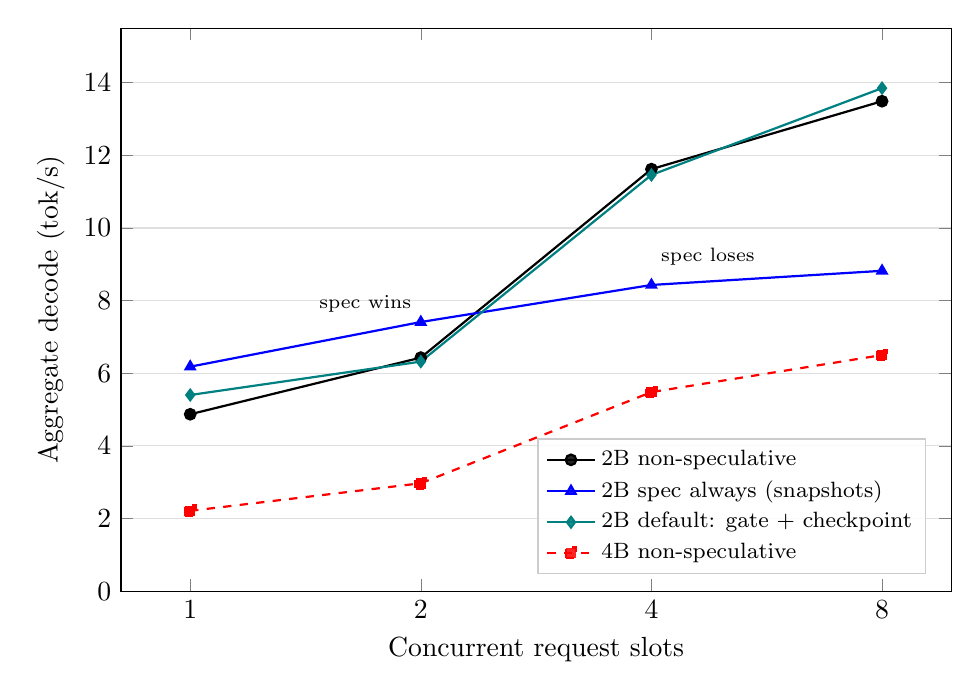
\begin{tikzpicture}
\begin{axis}[
  width=\columnwidth, height=0.72\columnwidth,
  xlabel={Concurrent request slots},
  ylabel={Aggregate decode (tok/s)},
  symbolic x coords={1,2,4,8},
  xtick=data,
  ymin=0, ymax=15.5,
  ymajorgrids=true, grid style={gray!25},
  legend style={at={(0.97,0.03)}, anchor=south east, font=\footnotesize, draw=gray!40, fill=white, fill opacity=0.85, text opacity=1},
  legend cell align={left},
  mark size=1.9pt,
  every axis plot/.append style={thick},
]
\addplot[color=black, mark=*] coordinates {(1,4.87) (2,6.43) (4,11.62) (8,13.49)};
\addlegendentry{2B non-speculative}
\addplot[color=blue, mark=triangle*] coordinates {(1,6.18) (2,7.41) (4,8.43) (8,8.82)};
\addlegendentry{2B spec always (snapshots)}
\addplot[color=teal, mark=diamond*] coordinates {(1,5.40) (2,6.32) (4,11.46) (8,13.85)};
\addlegendentry{2B default: gate + checkpoint}
\addplot[color=red, mark=square*, dashed] coordinates {(1,2.21) (2,2.97) (4,5.48) (8,6.50)};
\addlegendentry{4B non-speculative}
\node[font=\scriptsize, anchor=west] at (axis cs:4,9.2) {spec loses};
\node[font=\scriptsize, anchor=east] at (axis cs:2,7.9) {spec wins};
\end{axis}
\end{tikzpicture}
\caption{Aggregate decode throughput versus concurrency. Drafting always-on wins below the crossover and collapses above it; the default gate-plus-checkpoint configuration tracks the better side of both regimes.}
\label{fig:conc}
\end{figure}

\paragraph{Integrated build under concurrency.}
The sweep was repeated on the integrated build (mapped 32k d2t head plus the M4 scale rewrite) with the same English prompt; Table~\ref{tab:conc2} shows the results. Two findings stand out. First, the M4 scale rewrite improves \emph{batched} decode by about 5\% at 4--8 slots (12.20 versus 11.62; 14.17 versus 13.49) --- a gain invisible at one stream, because batched decode engages the M4 GEMM path that single-token decode never uses. Second, the crossover persists on the new build: with snapshot rollback enabled, multi-slot runs degrade even though only one slot drafts (5.48 at two slots versus 6.52 non-speculative), because snapshot maintenance taxes all slots. The checkpoint-plus-gate default and the n-gram-first drafter are both concurrency-neutral (13.77 and 13.91 at eight slots), so either can be enabled without giving up aggregate throughput.

\begin{table}[t]
\centering
\caption{Aggregate decode throughput (tok/s) on the integrated build (d2t mapped head + M4 scale), 2B.}
\label{tab:conc2}
\resizebox{\columnwidth}{!}{%
\begin{tabular}{lrrrr}
\toprule
Configuration & 1 slot & 2 slots & 4 slots & 8 slots \\
\midrule
Non-speculative & 4.92 & 6.52 & 12.20 & \textbf{14.17} \\
Default: gate + checkpoint & 5.21 & 6.30 & 11.46 & 13.77 \\
Spec + snapshots, gate=1 & \textbf{6.80} & 5.48 & 9.12 & 10.57 \\
N-gram-first + MTP & 5.20 & 6.31 & 11.81 & 13.91 \\
\bottomrule
\end{tabular}
}
\end{table}

\subsection{Hybrid dispatch and context costs}
The hybrid IME/RVV prototype regressed the 2B Q4\_0 pp64 result from 22.763 to 21.529 tok/s and tg32 from 5.149 to 2.006 tok/s. It was removed from the integrated patch set. Its implementation also duplicates weights, increasing model-weight memory demand by approximately a factor of two, an unattractive trade-off on a memory-constrained board.

The local 2B and 4B GGUFs declare a 262,144-token context, while the evaluated runtime setting was 8,192 tokens. Based on model metadata, estimated f16 attention KV storage at 8k is approximately 96 MiB for 2B and 256 MiB for 4B; at 16k it is approximately 192 MiB and 512 MiB. At one million tokens, the same estimate reaches about 11.4 GiB and 30.5 GiB, respectively, for attention KV alone. This excludes recurrent state, MTP state, allocator overhead, and other runtime memory. Accordingly, long-context systems such as windowed MTP or specialized KV-buffer schemes were not ported: the present 8k workload does not exercise their target bottlenecks, and one million tokens is outside both the model's declared context and the practical memory budget of the 16 GiB board.

\section{Discussion}
The optimization results separate into three classes. First, Q8\_0 IME1 unlocks a substantial prompt-processing improvement on a route that was poorly served by the baseline; the gain is specific to the 4B Q8\_0 case and does not imply that Q8\_0 is faster than Q4\_0. Second, M4 scale construction yields a small end-to-end benefit and is the most broadly useful low-risk kernel result in the evaluated Q4\_0 paths. Third, MTP policy and map changes are sensitive to draft cost, acceptance, and calibration quality; accepted-token rate alone is not enough to predict tokens per second.

The experiments also reinforce a measurement principle: report kernel throughput and end-to-end throughput separately. A kernel-level improvement can be correct and repeatable while total application throughput moves only slightly. Conversely, a promising acceptance statistic or warm-up estimate can produce a policy that reduces full-run throughput. Interleaved A/B runs and prompt/output checks improve confidence, but more repetitions and confidence intervals would be needed to establish small gains under varied board load.

\section{Limitations and reproducibility}
This is an engineering evaluation on one physical board, a limited set of model sizes, quantizations, and prompts. Output hash equality covers only the reported greedy prompts, not arbitrary inputs or stochastic decoding. The report does not claim statistical significance for the approximately 1.8--3.3\% improvements. Board thermal state, background load, compiler configuration, and llama.cpp revision can change performance. The integrated implementation was recorded on branch \texttt{codex/k1-integrated} at commit \texttt{a990751}; its patch helper and raw records are in the project tree. Reproduction should use the same model files, compiler settings, board conditions, and llama.cpp revision before generalizing these results.

\section{Conclusion}
On the tested MUSE-Pi-Pro SpaceMiT K1, enabling the Q8\_0 IME1 path produced the strongest measured improvement: 6.69 times higher 4B prompt throughput and 55.8\% higher generation throughput than the corresponding baseline, with matching greedy output hashes on three prompts. The M4 scale rewrite produced a 3.3\% prompt gain for 4B Q4\_0 and about 1.8\% on mapped 2B MTP English and Chinese, with matching acceptance counts and hashes. The vocabulary map did not improve held-out throughput consistently, while the speculative timing gate and hybrid dispatch regressed tested workloads and were excluded. These results favor targeted kernel improvements validated end-to-end, with speculative policies enabled only after their full draft-and-verify cost is accounted for.

\balance
\begin{thebibliography}{9}
\bibitem{llamacpp_q8_ime}
ggml-org, ``llama.cpp pull request \#28479: Q8\_0 IME1 kernel support.''
\url{https://github.com/ggml-org/llama.cpp/pull/28479}.

\bibitem{x60_scale_study}
OpenSolvers, ``Trimming the Block-Scale Tax in a SpaceMiT X60 IME int8$\times$int4 GEMM Kernel.''
\url{https://github.com/opensolvers/benchmarks/blob/main/papers/x60-ime-block-scale-optimization.md}.

\bibitem{learning_to_draft}
J. Zhang et al., ``Learning to Draft: Adaptive Speculative Decoding with Reinforcement Learning,'' arXiv:2603.01639, 2026.
\url{https://arxiv.org/abs/2603.01639}.

\bibitem{speculative_decoding}
Y. Leviathan, M. Kalman, and Y. Matias, ``Fast Inference from Transformers via Speculative Decoding,'' in \emph{Proceedings of ICML}, 2023.
\url{https://arxiv.org/abs/2211.17192}.

\bibitem{adasd}
``AdaSD: Adaptive Speculative Decoding for Efficient Language Model Inference,'' arXiv:2512.11280, 2025.
\url{https://arxiv.org/abs/2512.11280}.

\bibitem{qwen35_2b}
Qwen, ``Qwen3.5-2B model card''.
\url{https://huggingface.co/Qwen/Qwen3.5-2B}.

\bibitem{qwen35_4b}
Qwen, ``Qwen3.5-4B model card''.
\url{https://huggingface.co/Qwen/Qwen3.5-4B}.

\bibitem{spacemit_llama_docs}
SpacemiT, ``llama.cpp documentation and K1 inference support.''
\url{https://github.com/spacemit-com/llama.cpp}.
\end{thebibliography}
\end{document}
